\documentclass[12pt]{article}

\usepackage[portuguese]{babel}
\usepackage{float}
\usepackage{listings}
\usepackage[T1]{fontenc}
\usepackage{indentfirst}
\usepackage{amsfonts, amssymb, amsmath}
\usepackage{graphicx}
\usepackage{enumitem}
\usepackage[colorlinks=true, allcolors=blue]{hyperref}
\usepackage[letterpaper,
            top=1.5cm,
            bottom=1.5cm,
            left=2.75cm,
            right=2.75cm,
            marginparwidth=1.75cm]{geometry}

\title{Linguagens Formais e Autômatos}
\author{Prof. Yandre Costa}
\date{\today}

\begin{document}
\maketitle
Site do Professor: \url{http://www.din.uem.br/yandre} 
\section{Teoria da Computação}
\begin{itemize}[label=$\rightarrow$]
    \item Ciência da Computação
    \begin{itemize}
        \item Ênfase teórica: ideias fundamentais e modelos computacionais.
        \item Ênfase prática: projeto de sistemas computacionais.
    \end{itemize}
    \item A teoria da computação possui duas grandes vertentes.
    \begin{enumerate}
        \item Linguagens Formais e Autômatos.
        \item Máquinas Universais e Computabilidade.
    \end{enumerate}
    \item O que é Teoria da Computação?
    \begin{itemize}
        \item Estudos teóricos acerca da capacidade de resolução de problemas 
        das máquinas.
        \item Estudo de modelos formais que:
        \begin{itemize}
            \item Caracterizam em nível conceitual: programas, máquinas e enfim, 
            a computação.
            \item Especificam o que é computável ou não.
            \item Ajudam na especificação de linguagens artificiais entre outras 
            aplicações.
        \end{itemize}
    \end{itemize}
    \item Histórico da Computação
    \begin{itemize}
        \item Computar, do latim "computare", que significa calcular, avaliar, 
        contar.
    \end{itemize}
\end{itemize}

\section{Conceitos Básicos}
\begin{itemize}
    \item Introdução
    \begin{itemize}
        \item Problema: definir um conjunto de cadeias de símbolos
        \item Exemplo: conjunto \(M\) dos números bínários que têm 2 digitos
        \[ M=\{00,01,10,11\} \]
        \item Porém, se fosse o conjunto \(N\) de todas as combinações de 
        dígitos binários, poderiamos tentar o seguinte:
        \[ N=\{0,1,00,01,10,11,000,\dots\} \]
        \begin{itemize}
            \item Percebe-se que este conjunto é infinito
        \end{itemize}
        \item Representação clara: humanos x computador
        \item Representação formal: computador
        \item Um objetivo de LFA pe estudar uma maneira precisa e formal de 
        descrever sequencias de simbolos pertencentes a um determinado conjunto.
        \item Em especial conjuntos que não podem ser trivialmente enumerados.
        \item Os estudos iniciais foram em torno de Linguagens Naturais (LN).
        \item Algumas caracteristicas de LN introduziram dificuldades no 
        tratamento computacional das mesmas.
        \begin{itemize}
            \item LN é extensa, complexa, não tem sintaxe rígida e semântica 
            bem determinada (rica em ambiguidade)
        \end{itemize}
        \item As maneiras sistematicas de descrever uma linguagem de programação 
        são:
        \begin{itemize}
            \item Um método que permite construir programas sintaticamente 
            corretos - geração (Gramática)
            \item Um método que permite verificar se um programa escrito está 
            sintaticamente correto - reconhecimento (Autômatos)
        \end{itemize}
        \item Hierarquia de Chomsky
        \begin{figure}[H]
            \centering
            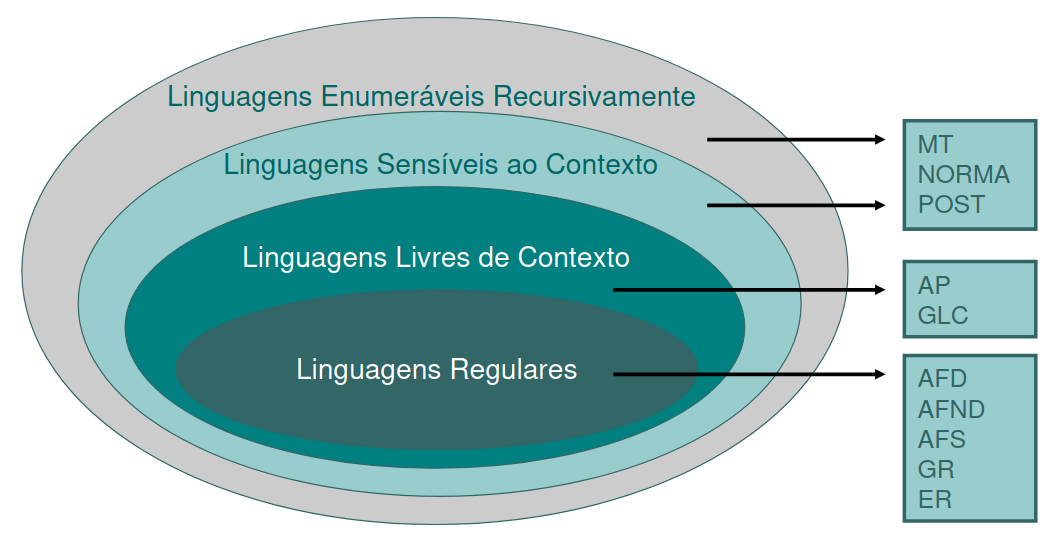
\includegraphics[width=0.75\linewidth]{imagens/hierarquia_chomsky.png}
        \end{figure}
        \item Pesquisas já demonstraram o uso destas tecnicas em:
        \begin{itemize}
            \item Análise de linguagens de programação
            \begin{itemize}
                \item Léxica
                \item Sintática
            \end{itemize}
            \item Modelos de sistemas biologicos
            \item Desenho de hardware
            \item Relacionamentos com linguagens Naturais
            \item Reconhecimento de padões (em visão computacional por exemplo)
        \end{itemize}
    \end{itemize}
    \item Alfabeto
    \begin{itemize}
        \item Conjunto de simbolos finito e não vazio
        \item Normalmente denotado por \(\Sigma\)
        \item Exemplos
        \begin{itemize}
            \item \(\Sigma=\{a,b\}\)
            \item \(\Sigma=\{1,2,3\}\)
            \item \(\Sigma=\{00,11\}\)
        \end{itemize}
    \end{itemize}
    \item Simbolo ou letra
    \begin{itemize}
        \item É todo elemento pertencente a um alfabeto
        \item \(a\) é um simbolo de \(\Sigma\)
    \end{itemize}
    \item Cadeia ou palavra
    \begin{itemize}
        \item É uma concatenação de simbolos do alfabeto justapostos.
        \item Assim, dado um alfabeto \(\Sigma\) e uma sequencia de simbolos 
        \(x=a_1a_2a_3\ldots a_n\), \(x\) é uma cadeia sobre \(\Sigma\) se, e 
        somente se, \(a_i\in\Sigma\) para \(i=1,2,\dots,n\).
        \item Comprimento de Cadeia ou Tamanho de Palavra
        \begin{itemize}
            \item É o numero de simbolos que compoem uma dada cadeia (ou palavra)
            \item O comprimento de uma cadeia $x$ é denotado por $|x|$
            \item Então, a cadeia \(x=a_1a_2a_3\ldots a_n\) tem seu comprimento 
            \(|x|=n\)
            \item Cadeia nula ou palavra vazia: é o caso especial, ela é 
            denotada por \(\lambda\) (ou \(\varepsilon\)) e tem o tamanho igual 
            a zero
            \item Exercicio: dado o alfabeto \(\Sigma={a,b,c,de}\), verifique 
            se as cadeias a seguir são formadas sobre este alfabeto, e se for, 
            verifique qual o comprimento 
        \end{itemize}
    \end{itemize}
    \item Exponenciação de Alfabetos
    \begin{itemize}
        \item \(\Sigma^k\) é o conjunto de todas as cadeias com tamanho \(k\) 
        formadas sobre o alfabeto \(\Sigma\)
        \item Exemplo: Considere \(\Sigma=\{0,1\}\)
        \begin{itemize}
            \item \(\Sigma^0 = \lambda\)
            \item \(\Sigma^1 = \{0,1\}\)
            \item \(\Sigma^2 = \{00,01,10,11\}\)
            \item \(\Sigma^3 = \{000,001,010,011,100,101,110,111\}\)
        \end{itemize}
    \end{itemize}
    \item Fechamento de um Alfabeto
    \begin{itemize}
        \item Seja $\Sigma$ um alfabeto, então, o fechamento de $\Sigma$ 
        descrito por $\Sigma^*$ é definido como
        \[ \Sigma^*= \Sigma^0 \cup \Sigma^1 \cup \Sigma^2 \cup \ldots \cup 
        \Sigma^n \cup \ldots\] 
    \end{itemize}
    \item Concatenação de cadeias
    \begin{itemize}
        \item Dado o alfabeto \(\Sigma\) e as cadeias \(x,y \in \Sigma^*\), a 
        concatenação de \(x\) e \(y\), indicada por \(xy\), produz uma cadeia 
        formada pelos simbolos de \(x\) seguidos pelos simbolos de \(y\).
        \item Se \(x=a_1a_2a_3 \ldots a_n \in \Sigma^* \) e \(y=b_1b_2b_3 
        \ldots b_m \in \Sigma^* \) então: 
        \[xy=a_1a_2a_3 \ldots a_nb_1b_2b_3 \ldots b_m \]
        \item Exemplos:
        \begin{itemize}[label=]
            \item \(\Sigma=\{a,b\}\)
            \item \(x=abaa, y=ba, z=\lambda\)
            \item \(xy=abaaba\)
            \item \(yx=baabaa\)
            \item \(yz=ba=zy=y\)
        \end{itemize}
        \item A cadeia nula (\(\lambda\)) é o elemento neutro da concatenação
        \item Concatenação Sucessiva -- Concatenação de uma palavra com ela 
        mesma.
        \begin{itemize}
            \item Representada através de um expoente: \(w^n\) -- Onde \(w\) é 
            uma palavra e \(n\) indica o número de concatenações sucessivas.
        \end{itemize}
    \end{itemize}
    \item Dado um alfabeto $\Sigma$ e $x,y\in\Sigma^*$, diz-se que:
    \begin{itemize}
        \item $x$ é um prefixo de $y$, se e somente se, $\exists w\in\Sigma^*$ 
        tal que $y=xw$
        \item $x$ é um sufixo de $y$, se e somente se, $\exists w\in\Sigma^*$ 
        tal que $y=wx$
        \item $x$ é uma subpalavra de $y$, se e somente se, $\exists w,u\in
        \Sigma^*$ tal que $y=wxu$
    \end{itemize}
    \item Linguagem
    \begin{itemize}
        \item Dado o alfabeto $\Sigma$, o conjunto de palavras $L$ é uma 
        linguagem sobre $\Sigma$ se e somente se $L \subset \Sigma^*$.
        \item Operações sobre linguagens:
        \begin{itemize}
            \item Considere \(L_1\) e \(L_2\) linguagens definidas sobre 
            \(\Sigma\)
            \begin{itemize}
                \item União: \(L_1 \cup L_2 = \{x|x\in L_1 \vee x \in L_2\}\)
                \item Interseção: \(L_1 \cap L_2 = \{x|x\in L_1 \wedge x \in 
                L_2\}\)
                \item Diferença: \(L_1 - L_2 = \{x|x\in L_1 \wedge x \notin 
                L_2\}\)
                \item Concatenação: \(L_1L_2 = \{x|x=yz, y \in L_1 \wedge z \in 
                L_2\}\)
                \item Complemento: \(\bar{L_1} = \{x|x\in \Sigma^* \wedge x 
                \notin L_1\}\)
            \end{itemize}
        \end{itemize}
    \end{itemize}
    \item Comparando as definições:
    \begin{itemize}
        \item Linguagem Natural:
        \begin{itemize}
            \item Uma palavra em portugues equivale a um simbolo
            \item Uma sentença da lingua portuguesa é uma cadeia composta de 
            vários simbolos.
        \end{itemize}
        \item Linguagem computacional
        \begin{itemize}
            \item Cada programa escrito numa linguagem computacional corresponde 
            a uma cadeia de simbolos que podem ser:
            \begin{itemize}
                \item Identificadores;
                \item Palavras reservadas;
                \item Simbolos especiais e operadores;
                \item Constantes numéricas.
            \end{itemize}
        \end{itemize}
    \end{itemize}
\end{itemize}
\section{Autômatos Finitos}
\begin{itemize}
    \item AFD -- Modelo matmático para definição de linguagem
    \item Caráter reconhecedor
    \item Modelam também sistemas de estados finitos
    \item Exemplo clássico: problema HLCR (Hopcroft e Ullman)
    \vspace{32pt}
    \item Problema: um homem quer atravessar um rio levando consigo um lobo, uma 
    cabra e um repolho, e no bote, só cabem ele e mais um dos outros três.
    \item Exemplos de possiveis estados do sistema:
    \begin{itemize}
        \item <HLCR-0> -- todos na margem esquerda
        \item <L-HCR> -- lobo na margem esquerda, cabra e repolho na direita
    \end{itemize}
    \item Entradas do sistema:
    \begin{itemize}
        \item h -- Homem atravessa o rio sozinho
        \item l -- Homem atravessa o rio com o lobo
        \item c -- Homem atravessa o rio com a cabra
        \item r -- Homem atravessa o rio com o repolho
    \end{itemize}
    \item Objetivo: <HLCR-0> $\Rightarrow$ <0-HLCR>
    \item Representação por diagrama:
    \begin{itemize}
        \item Circulos representam estados
        \item Arcos representam ação ou transição (de um estado para o outro)
        \item O estado final é marcado por um circulo duplo
        \item As respostas para o problema são as sequências de ações que 
        levam do estado inicial para o final
    \end{itemize}
\end{itemize}
    \subsection{Autômato Finito Determinístico}
    \begin{itemize}
        \item Exemplo de sistema que pode ser representado desta forma: 
        \begin{itemize}
            \item Forno de micro-ondas
            \begin{itemize}
                \item Entradas: porta aberta ou fechada, comandos fornecidos 
                pelo cozinheiro através do painel, sinal do "timer" que expira 
                \item Estados: aberto, esperando por comandos, cozinhando, 
                desligado
            \end{itemize}
        \end{itemize}
        \item Definições Básicas
        \begin{itemize}
            \item Um AFD $A$ define uma linguagem $L(A)$ sobre um alfabeto $\Sigma$
            \item Caráter reconhecedor, ao contrário das gramáticas estudadas 
            que tinham caráter gerador
            \begin{itemize}
                \item Dada uma cadeia $x$, ela pertence a $L(A)$
            \end{itemize}
            \item Uma abstração de um AFD
            \begin{itemize}
                \item Uma cabeça de leitura extrai sequencialmente o conteúdo 
                de uma fita (string)
                \item Uma luz de aceitação que acende somente se a cadeia 
                pertencer a linguagem representada pela AFD
                \item Exemplos de cadeias aceitas em HLCR
                \begin{itemize}
                    \item chrclhc, ccchllrclllhccc, \ldots
                \end{itemize}
            \end{itemize}
            \item Definição Matemática de um AFD
            \begin{itemize}
                \item Uma AFD é uma quintupla $<\Sigma, S, S_0, \delta, F>$, 
                onde:
                \begin{itemize}
                    \item $\Sigma$ é o alfabeto de Entradas
                    \item $S$ é um conjunto finito não vazio de estados
                    \item $S_0$ é o estado inicial, $S_0 \in S$
                    \item $\delta$ é a funçã de transição de estados, definida 
                    $\delta:S \times \Sigma \rightarrow S $
                    \item $F$ é o conjunto de estados finais, $F \subseteq S$
                \end{itemize}
                \item Uma cadeia $x$ para ser aceito, deve levar do estado $S_0$ 
                para algum estado pertencente a $F$
                \item A função $\delta$ determina como são as transições de 
                estados. Ela leva um par $<s,a>$ onde $s$ é um estado e $a$ uma 
                letra do alfabeto num estado $s'$ 
                \begin{itemize}
                    \item $\delta(s,a)=s'$
                \end{itemize}
                \item Então, dado um AFD $A=<\Sigma, S, S_0, \delta, F>$ e a 
                cadeia $x=a_1a_2a_3\ldots a_n \in \Sigma^*$, o autômato parte 
                de $S_0$. Ao processar $a_1$ passa para o estado $\delta 
                (S_0,a_1)$, ao processar $a_2$ passa para o estado $\delta 
                (S_0,a_2)$, e assim por diante até processar $a_n$. Nesse ponto, 
                o autômato estará num estado $R$ qualquer. Se $R \in F$, então 
                a cadeia $x \in L(A)$.
                \item Finito: númeto de estados envolvidos no sistema é finito
                \item Determinístico: Estabelece que para uma cadeia $x \in 
                L(A)$, só existe uma única sequencia de estados no AFD $A$ para 
                preocessá-la.
            \end{itemize}
        \end{itemize}
        \item Exercicios
        \begin{itemize}
            \item Dados os seguintes autômatos:
            
            \item Identifique a linguagem associada a cada um
            \begin{itemize}[label=R:]
                \item Autômato 1: $L=\{a^nbc^m \vee a^ncb^m | n \geq 0, m \geq 0\}$ \\
                Autômato 2: $L=\{aa^nbb^m | n \geq 0, m \geq 0\}$ \\
                Autômato 3: $L=\{a..zA..Z(a..zA..Z0..9)^n | n \geq 0\}$
            \end{itemize}
            \item Descreva as funções de transição de cada um (exceto para o 
            terceiro diagrama)
            \begin{itemize}[label=R:]
                \item Autômato 1: 
                \[\delta(S_0,a)=S_0; \delta(S_0,b)=S_1; \delta(S_1,c)=S_1\] 
                \begin{center}OU\end{center} 
                \[\delta(S_0,a)=S_0; \delta(S_0,c)=S_2; \delta(S_2,b)=S_2\] \\
                Autômato 2: \[ \delta(S_0, a)=S_1; \delta(S_1, a)=S_1; 
                \delta(S_1, b)=S_2; \delta(S_2,b)=S_2 \]
            \end{itemize}
        \item Exemplo:
        \begin{itemize}
            \item Modelagem de uma "vending machine" que aceita moedas de 5, 
            10 e 25 centavos. O preço do produto que ela entrega é 30 centavos.
            \item Partindo do estado inicial (0 centavos), deveremos reconhecer 
            sequencias que nos levem a estados finais (valor inserido $\geq$ 30 
            centavos)
            \item Podemos chamar o autômato de $V$
            \item Assim:
            \begin{itemize}
                \item $V=<\Sigma, S, S_0, \delta, F>$ onde:
                \item $\Sigma=\{5,10,25\}$ -- Cada um destes símbolos (ou letras) 
                representa uma ação.
                \item $S=\{<0c>,<5c>,<10c>,<15c>,<20c>,<25c>,<30c>,<35c>,<40c>,
                <45c>,<50c>\}$ -- Cada estado indica quanto foi depositado.
                \item $S_0 = <0c>$ -- estado inicial.
                \item $F = \{<30c>,<35c>,<40c>,<45c>,<50c>\}$ -- estado onde a 
                entrada é válida e o produto pode ser liberado.
                \item Delta é definido como: 
                \begin{center}
                        $\delta(<0c>, 5)=<5c>$ \\
                        $\delta(<0c>, 10)=<10c>$ \\
                        $\delta(<0c>, 25)=<25c>$ \\
                        $\delta(<5c>, 5)=<10c>$ \\
                        $\delta(<5c>, 10)=<15c>$ \\
                        $\delta(<5c>, 25)=<30c>$ \\
                        $\delta(<10c>, 5)=<15c>$ \\
                        \dots
                \end{center}
                \item Tabela de transição de estados
                \begin{table}[H]
                    \centering
                    \begin{tabular}{|c|ccc|}
                        \hline
                        $\delta$ & 5 & 10 & 25 \\ \hline 
                        $<0c>$ & $<5c>$ & $<10c>$ & $<25c>$ \\
                        $<5c>$ & $<10c>$ & $<15c>$ & $<30c>$ \\ 
                        $<10c>$ & $<15c>$ & $<20c>$ & $<35c>$ \\ 
                        $<15c>$ & $<20c>$ & $<25c>$ & $<40c>$ \\ 
                        $<20c>$ & $<25c>$ & $<30c>$ & $<45c>$ \\ 
                        $<25c>$ & $<30c>$ & $<35c>$ & $<50c>$ \\ 
                        $<30c>$ & - & - & - \\ 
                        $<35c>$ & - & - & - \\ 
                        $<40c>$ & - & - & - \\ 
                        $<45c>$ & - & - & - \\ 
                        $<50c>$ & - & - & - \\ 
                        \hline
                    \end{tabular}
                \end{table}
                A tabela de transição é boa para demonstrar transições 
                grandes, e tambem para implementar em codigos, usando uma 
                matriz para descrever a tabela de transição!! \\
                Para descrevermos que a quantia de itens é a definição de 
                um AFD, podemos dizer, por exemplo, que 
                $L=\{x \in \Sigma^* | |x|_a \text{condição} \}$
                \end{itemize}
            \end{itemize}
        \end{itemize}
    \end{itemize}
    \subsection{Autômato Finito Não Deterministico -- AFND}
    \begin{itemize}
        \item Modelo matemático semelhante ao AFD
        \item Condições mais flexiveis
        \item Podem haver multiplos caminhos para processar uma cadeia
        \item Definição formal
        \begin{itemize}
            \item Uma AFD é uma quintupla $<\Sigma, S, S_0, \delta, F>$, 
                    onde:
            \begin{itemize}
                \item $\Sigma$ é o alfabeto de entradas
                \item $S$ é um conjunto finito não vazio de estados
                \item $S_0$ é um conjunto não vazio de estados iniciais, $S_0 
                \subseteq S$
                \item $\delta$ é a função de transição de estados, definida 
                $\delta:S \times \Sigma \rightarrow \rho(S)$
                \begin{itemize}
                    \item A função pode ativar todos os possiveis subconjuntos 
                    dos estados
                \end{itemize}
                \item $F$ é o conjunto de estados finais, $F \subseteq S$
            \end{itemize}
            \item $\Sigma, S$ e $F$ são os mesmos do AFD;
            \item $S_0$ era um unico estado em AFD. Em AFND é um conjunto com 
            pelo menos um estado inicial
            \begin{itemize}
                \item Então em AFD, $S_0 \in S$, e em AFND, $S_0 \subseteq S$
            \end{itemize}
            \item Um AFND pode ter mais de um estado "ativo" (corrente) num 
            instante;
            \item Inicialmente, todo estado de $S_0$ são ativados;
        \end{itemize}
        \item "Alternativas" para processar uma unica cadeia;
        \item Se o processamento de uma cadeia não levar ao estado final por um 
        caminho, deve-se tentar por outros caminhos (se houverem);
        \item Se algum dos caminhos possiveis levar a cadeia $x$ a um estado 
        final, então ela faz parte da linguagem definida pelo automato.
        \item A cadeia é rejeitada se a partir de nenhum estado inicial for 
        possivel atingir um estado final ao termino do processamento;
        \item A função $\delta$ agora é definida por $S \times\Sigma\rightarrow
        \rho(S)$
        \item Exemplo da função $\delta(S,a)={R,T}$
        \item[] imagem
        \item Se o estado $S$ estiver ativo e a letra $a$ for processada, então 
        tanto $R$ quanto $T$ passaram a estar ativos;
        \item Se seguirmos por $R$ e não chegarmos a um estado final, podemos 
        tentar por $T$
        \item Se alguma das alternativas levar a um estado final, a cadeia é 
        reconhecida
        \item Se nenhuma alternativa levar a um estado final, a cadeia é rejeitada;
        \item Ao processar uma letra, todas as transições rotuladas com aquela 
        letra, a partir de todos os estados ativos serão efetuadas
        \item Então, podemos novamente observar que podemos ter vários estados 
        ativos ao mesmo tempo, ao contrário dos AFDs
    \end{itemize}
    \subsection{Equivalência entre AFD e AFND}
    \begin{itemize}
        \item A classe dos AFDs é equivalente à classe doas AFNDs. Assim, para 
        todo AFD existe um AFND equivalente e vice-versa.
        \item Exemplo -- $L(A)=\{ w|w\in \{a,b\}^* \wedge w \text{possui aaa 
        como sufixo} \}$
        \item[] imagem
        \item Exercicio
        \begin{itemize}
            \item Construa um AFD e um AFND para a seguinte linguagem:
            \begin{itemize}
                \item \( L(A)=\{w|w \in {a,b}^* \wedge w\} \) possui $aa$ como 
                subpalavra
                \item[] imagem 
            \end{itemize}
        \end{itemize}
        \item Transformação de AFND em AFD
        \begin{itemize}
            \item Para todo AFND existe um AFD equivalente
            \item Dado um AFND $A = <\Sigma, S, S_0, \delta, F>$, define-se 
            o AFD $A^d = <\Sigma, S^d, S^d_0, \delta^d_0, F^d>$ equivalente da 
            seguinte forma:
            \begin{itemize}
                \item $S^d = \rho(S)$
                \item $S^d_0=S_0$
                \item $F^d$: Todas as combinações de estados de $S^d$ que possui 
                como componente algum estado de $F$
                \item Seja $Q\in S^d$, $\delta^d(Q,a)$ vai levar à um estado 
                que corresponde à combinação de todos os estados que podem ser 
                alcançados ao processar o simbolo '$a$' a partir de qualquer 
                componente $Q$
            \end{itemize}
            \item Exemplo 1:
            \begin{itemize}
                \item Dado o AFND:
                \item [] imagem
                \item Cria um estado para cada combinação possivel de estados 
                do AFND
                \item Estabelece-se como estado inicial a combinação 
                correspondente ao conjunto de estados iniciais do AFND
                \item Estados finais: todos que possuem em sua combinação algum 
                dos estado finais do AFND
                \item Criação das transições:
                \begin{itemize}
                    \item $\delta^d(Q,a)$ será igual ao estado que corresponda 
                    à combinação de todos os estados que formam o conjunto 
                    $\delta(Q,a)$
                    \item[] imagem
                \end{itemize}
            \end{itemize}
            \item Durante a transformaçãp de um AFND em um AFD podem ser criados 
            estados que fiquem "isolados" do(s) estado(s) inicial(is)
            \item Exercicio: Transforme o AFND descrito a seguir em um AFD
            \item [] imagem
        \end{itemize}
        \item Minimização de AFD
        \begin{itemize}
            \item Dois AFDs $A$ e $B$ são equivalentes, denotado por $A 
            \equiv B$, se $L(A) = L(B)$
            \item Um automato minimo para uma linguagem regular L é um 
            automato com o menor numero de estados possivel que aceita $L$
            \begin{itemize}
                \item Um AFD $A = <\Sigma, S_A, S_{0A}, \delta_A, F_A>$ é 
                dito minimo se para qualquer AFD $B = <\Sigma, S_B, S_{0B}, 
                \delta_B, F_B>$ tal que $A \equiv B$, temos que $|S_A|\leq
                |S_B|$
            \end{itemize}
            \item Pré-requisitos para a minimização:
            \begin{itemize}
                \item O automato deve ser Deterministico
                \item Não pode ter estados inacessiveis a partir do estado 
                inicial
                \item A função de transição deve ser total (todas as saídas 
                devem ser previstas para todos os estados)
                \begin{itemize}
                    \item Para este ultimo requisito muitas vezes é necessario 
                    introduzir um estado $S_\text{trash}$ para lançar as 
                    transições não previstas originalmente
                \end{itemize}
            \end{itemize}
            \item A estratégia consiste em fundir estados equivalentes num mesmo 
            estado
            \begin{itemize}
                \item Dois estados são equivalentes se, ao processarem uma mesma 
                cadeia, ambos chegam a estados finais, ou ambos chegam a estados 
                não finais
            \end{itemize}
            \item Para isto, são identificados estados não-equivalentes e, por 
            exclusão, encontra-se os equivalentes
            \item Utiliza-se uma tabela triangular que possui um cruzamento para 
            cada par de estados distintos do automato (incluindo $S_\text{trash}$ 
            quando este é acrescentado)
            \item Supondo um autômato com $S=\{S_0,S_1, \dots, S_{n-1}, S_n, 
            S_\text{trash}\}$ 
            \item [] imagem
            \begin{itemize}
                \item Estados não equivalentes serão sinalizados, ao final do 
                processo, os cruzamentos em branco deverão indicar estados 
                equivalentes.
            \end{itemize}
            \item Inicia-se a marcação pelos estados trivialmente não-equivalentes
            \begin{itemize}
                \item Dois estados não trivialmente não-equivalentes se um é 
                final e o outro não
            \end{itemize}
            \item Exemplo:
            \begin{itemize}
                \item Considere o seguinte AFD e sua tabela de cruzamento de estados
                \item[] imagem
                \item[] \dots
            \end{itemize}
            \item Critério usado para a marcação dos estados não equivalentes:
            \begin{itemize}
                \item Para cada par $\{S_u,S_v\}$ não marcado e para cada 
                simbolo $a \in \Sigma$, suponha que $\delta(S_u,a)=R_u$ e 
                $\delta(S_v,a)=R_v$
                \begin{itemize}
                    \item Se $R_u=R_v$, então $S_u$ e $S_v$ são equivalentes e, 
                    para o simbolo $a$ não deve ser marcado
                    \item Se $R_u \neq R_v$, e o par $\{R_u,R_v\}$ não está 
                    marcado, então $\{S_u,S_v\}$ é incluido em uma lista a 
                    partir de $\{R_u,R_v\}$ para posterior analise
                    \item Se $R_u \neq R_v$, e o par $\{R_u,R_v\}$ está 
                    marcado, então:
                    
                    $\rightarrow$ $\{S_u,S_v\}$ é não equivalente e deve ser
                    marcado

                    $\rightarrow$ Se $\{S_u,S_v\}$ encabeça uma lista de pares, 
                    então todos os pares da lista devem ser marcados
                \end{itemize}
            \end{itemize}
            \item Na unificação dos estados equivalentes:
            \begin{itemize}
                \item Conjuntos de estados finais equivalentes podem ser 
                unificados como um unico estado final
                \item Conjuntos de estados não-finais equivalentes podem ser 
                unificados como um unico estado não-final
                \item Se algum dos estados equivalentes é inicial, então o 
                correspondente estado unificado é inicial
            \end{itemize}
        \end{itemize}
    \end{itemize}
\section{Expressões Regulares}
\begin{itemize}
    \item Formalismo de carater gerador
    \begin{itemize}
        \item A partir dee pode-se inferir como construir as cadeias da linguagem
    \end{itemize}
    \item Pode representar qualquer LR -- Linguagem Regular
    \item Uma ER é definida a partir de conjuntos básicos e operadores de 
    concatenação e união 
    \item Formalismo adequado para comunicação homem $\times$ homem e homem 
    $\times$ máquina
    \item Uma ER sobre um alfabeto $\Sigma$ é definida como segue:
    \begin{itemize}
        \item $\varnothing$ é uma ER e denota a linguagem vazia
        \item $\varepsilon$ é uma ER e denota a linguagem contendo exclusivamente 
        a palavra vazia, ou seja, $\{\varepsilon\}$
        \item Qualquer simbolo $x$ pertence a $\Sigma$ é uma ER e denota a 
        linguagem contendo a palavra $x$, ou seja, $\{x\}$
        \item Se $r$ e $s$ são ERs e denotam as linguagens $R$ e $S$, 
        respectivamente, então:
        \begin{itemize}
            \item $(r+s)$ é ER e denota a linguagem $R \cup S$ (União)
            \item $(rs)$ é ER e denota a linguagem $RS=\{uv|u\in R \text{ e } 
            v \in S\}$ (Concatenação)
            \item $(r^*)$ é ER e denota a linguagem $R^*$ (Fecho)
        \end{itemize}
        \item Pode-se utilizar parenteses ou não, mas deve-se considerar a 
        seguinte convenção:
        \begin{itemize}
            \item A concatenação sucessiva (fechamento ou fecho de Kleene) tem 
            precedencia sobre a concatenação
            \item A concatenação tem precedência sobre a união
        \end{itemize}
        \item Exemplos de ER
        \item[] Tabela
    \end{itemize}
    \item ERs podem ser usadas em buscas em editores de texto

\end{itemize}

\section{Gramática}
\begin{itemize}
    \item Mecanismo gerador que permite definir formalmente uma linguagem
    \item Através de uma gramática pode-se gerar todas as sentenças da linguagem 
    definida por ela
    \item Modelo muito aplicado na especificação de linguagens computacionais
    \item Formalmente, gramática é uma quadrupla $G = (V,T,P,S)$ onde:
    \begin{itemize}
        \item $V$ é um conjunto finito de símbolos não-terminais (ou variáveis)
        \item $T$ é um conjunto finito de símbolos terminais disjunto de $V$
        \item $P$ é um conjunto finito de pares, denominados regras de produção 
        tal que a primeira componente é uma palavra de $(V\cup T)^+$ e a segunda 
        componente é uma palavra $(V\cup T)^*$
        \item $S$ é um elemento de $V$, denominado símbolo inicial (ou símbolo 
        de partida)
    \end{itemize}
    \item Os símbolos de $T$ equivalem aqueles que aparecem nos programas de 
    uma linguagem de programação. É o alfabeto em cima do qual a linguagem é 
    definida 
    \item Os elementos de $V$ são símbolos auxiliares que são criados para 
    permitir a definição das regras da linguagem. Eles correspondem à 
    "catergorias sintáticas" da linguagem definida
    \begin{itemize}
        \item Português: sentença, predicado, verbo, \ldots;
        \item Pascal: programa, bloco, procedimento, \ldots;
    \end{itemize}
    \item Uma regra de produção $(\alpha, \beta)$ é representada por $\alpha 
    \rightarrow \beta$ 
    \item As regras de produção definem as condições de geração das sentenças
    \item A aplicação de uma regra de produçãp é denominada derivação
    \item Uma regra $\alpha \rightarrow \beta$ indica que $\alpha$ pode ser 
    substituído por $\beta$ sempre que $\alpha$ aparecer
    \item Enquanto houver símbolo não-terminal na cadeia em derivação, esta 
    derivação não terá terminado
    \item O simbolo inicial é o simbolo através do qual deve iniciar o processo 
    de derivação de uma sentença
    \item Observações:
    \begin{itemize}
        \item $V \cap T = \varnothing$
        \item Os elementos de $T$ são os terminais. Procuraremos representá-los 
        por letras minúsculas (a,b,c,d, \ldots)
        \item Os elementos de $V$ são os não-terminais. Procuraremos 
        representá-los por letras maiúsculas (A,B,C,D, \ldots)
        \item As cadeias mistas, isto é, aquelas que contém simbolos de $V$ e 
        simbolos de $T$ (cadeias pertencentes à $(V \cup T)^*$) serão 
        representadas por letras gregas ($\alpha$, $\beta$, $\gamma$, $\delta$, 
        \ldots)
    \end{itemize}
    \item Exemplo:
    \begin{itemize}
        \item $G_1 = (\{S,A,B\}, \{a,b\}, P, S)$ onde:
        \begin{itemize}
            \item $P = \{1) S \rightarrow AB \\
            2) A \rightarrow a \\
            3) B \rightarrow b\}$
        \end{itemize}
        \item Quais as cadeias terminais geradas por esta gramática?
        \begin{itemize}[label=R:]
            \item $ab$
        \end{itemize}
    \end{itemize}
    \item Descrição de linguagens:
    \begin{enumerate}
        \item $G_1 = (\{A,B\}, \{a,b,c\}, P, A)$ onde:
        
            $P = \{1) A\rightarrow aB \\
                2) B \rightarrow bB \\
                3) B \rightarrow c \}$

        \item $G_2 = (\{S,A,B,C\}, \{a,b,c\}, P, S)$ onde:
        
            $P = \{1) S\rightarrow A \\
                2) A \rightarrow BaC \\
                3) B \rightarrow bB \\
                4) B \rightarrow b \\
                5) C \rightarrow cC \\
                6) C \rightarrow c\}$
    \end{enumerate}
    \begin{itemize}
        \item A linguagem gerada pela gramática $G_1$ descrita acima, poderia 
        ser expressa da seguinte forma: $L(G_1) = \{ab^nc, n \geq 0\}$
        \item A linguagem gerada pela gramática $G_2$ descrita acima, poderia 
        ser expressa da seguinte forma: $L(G_2) = \{b^mac^n, m \geq 1, n \geq 1\}$
    \end{itemize}
    \item Geração direta ($\Rightarrow$):
    \begin{itemize}
        \item Considere $\alpha, \beta, \gamma, \delta \in (V \cup T)^*$
        \item Uma cadeia $\alpha\gamma\beta$ gera diretamente ($\Rightarrow$) 
        uma cadeia $\alpha\delta\beta$ se e somente se: 
        \[\gamma \rightarrow \delta \in P\]
    \end{itemize}
    \item Geração ($\Rightarrow^*$):
    \begin{itemize}
        \item Uma cadeia $\alpha$ gera ($\Rightarrow^*$) uma cadeia $\beta$ se 
        e somente se:
        \[\exists \gamma_1,\gamma_2, \ldots, \gamma_n | \alpha \rightarrow 
        \gamma_1 \rightarrow \gamma_2 \rightarrow \ldots \rightarrow \gamma_n 
        \rightarrow \beta, n \geq 0\]
    \end{itemize}
    \item Definições:
    \begin{itemize}
        \item Forma sentencial: uma cadeia $\alpha \in (V \cup T)^*$ é uma 
        forma sentencial de uma gramática se e somente se $S \Rightarrow^* 
        \alpha$, ou seja, $\alpha$ é um "embrião" para alguma sentença gerada 
        pela gramática ou a própria sentença
        \item Sentença: uma fora sentencial $\alpha$, é uma sentença de $G$ se 
        e somente se $\alpha \in T^*$. Portanto, as cadeias terminais geradas 
        pela gramática são as sentenças de $G$
    \end{itemize}
    \item Tipos de Gramática
    \begin{itemize}
        \item A cada classe de linguagem da Hierarquia de Chomsky é associado 
        um tipo de gramática
        \item Gramática com Estrutura de Frase -- GEF ou Tipo 0
        \begin{itemize}
            \item São as gramáticas onde todas as regras de produção 
            pertencentes ao conjunto P são da forma:
            \[
            \alpha \rightarrow \beta \text{ onde } \beta \in (V\cup T)^* \wedge \\
                                                \alpha \in (V\cup T)^+
            \]
            \item Os próximos tipos de gramática são GEFs com restrições
        \end{itemize}
        \item Gramática Sensivel ao Contexto -- GSC ou Tipo 1
        \begin{itemize}
            \item São as gramáticas onde todas as regras de produção 
            pertencentes ao conjunto $P$ são da forma:
            \[
            \alpha \rightarrow \beta \text{ tal que }|\beta|\geq |\alpha| 
            \text{ exceto quando } \beta = \lambda \]
            \[
            \beta \in (V\cup T)^* \]
            \[
            \alpha \in (V\cup T)^+
            \]
            \item Exemplo:
            
            \( S \rightarrow aSBC \\
            S \rightarrow aBC \\
            CB \rightarrow BC \\
            aB \rightarrow ab \\
            bB \rightarrow bb \\
            bC \rightarrow bc \\
            cC \rightarrow cc \)

            Gera a linguagem: $L(G) = \{a^nb^nc^n|n\geq 0\}$
        \end{itemize}
        \item Gramática Livre de Contexto -- GLC ou Tipo 2
        \begin{itemize}
            \item São as gramáticas onde todas as regras de produção pertencentes 
            ao conjunto $P$ são da forma:
            \[A \rightarrow \beta \text{ onde } \]
            \[\beta \in (V\cup T)^*\]
            \[A \in V\]
            \item Exemplos:
            \begin{itemize}
                \item \(S \rightarrow AB \\
                    A \rightarrow 0A11 \\
                    A \rightarrow \lambda \\
                    B \rightarrow 0B \\
                    B \rightarrow \lambda\)
                \item \(S \rightarrow aB \\
                    S \rightarrow bA \\
                    A \rightarrow a \\
                    A \rightarrow aS \\
                    A \rightarrow bAA \\
                    B \rightarrow b \\
                    B \rightarrow bS \\
                    B \rightarrow aBB\)
            \end{itemize}
            \item O próximo tipo de gramática é GLC com restrições
        \end{itemize}
        \item Gramática Regular -- GR ou Tipo 3
        \begin{itemize}
            \item Uma linguagem regular é uma linguagem que pode ser descruta 
            por uma gramática linear
            \item Tipos de gramática linear:
            \begin{itemize}
                \item Gramática Linear à Direita -- GLD
                \item Gramática Linear à Esquerda -- GLE
                \item Gramática Linear Unitária à Direita -- GLUD
                \item Gramática Linear Unitária à Esquerda -- GLUE
            \end{itemize}
            \item Seja $G = (V,T,P,S)$ e sejam $A$ e $B$ elementos de $V$, e 
            $w$ uma cadeia de $T^*$, então:
            \begin{itemize}
                \item GLD -- $A \rightarrow wB \vee A \rightarrow w$
                \item GLE -- $A \rightarrow Bw \vee A \rightarrow w$
                \item GLUD -- $A \rightarrow wB \vee (A \rightarrow w \wedge |w| 
                \leq 1)$
                \item GLUE -- $A \rightarrow Bw \vee (A \rightarrow w \wedge |w| 
                \leq 1)$
            \end{itemize}
        \end{itemize}
    \end{itemize}
\end{itemize}


\section{Algoritmo de reconhecimento para LLC}
\begin{itemize}
    \item Algoritmo de Cocke-Younger-Kasami
    \begin{itemize}
        \item Desenvolivdo independentemente por Cocke, Younger e Kasami em 1965
        \item Trabalha sobre uma GLC na Forma Normal de Chomsky (pré-requisito)
        \begin{itemize}
            \item Portanto, o algoritmo atende LLCs que não possuem a palavra 
            vazia
        \end{itemize}
        \item Realiza uma analise ascendente (bottom-up) das cadeias
        \item O algoritmo parte da cadeia a ser analisada e regride nas produções 
        formando uma tabela triangular
        \item Quando o triangulo estiver completo, a cadeia é aceita se o simbolo 
        de partida da gramatica estiver no topo do mesmo
        \item O estado inicial precisa estar no topo da tabela
        \item Considerando as dimensões "r" e "s" da tabela, conforme ilustra 
        a figura a seguir:
        \begin{enumerate}
            \item Regressão dos terminais
            \item Regressão dos não terminais
        \end{enumerate}
    \end{itemize}
\end{itemize}

\section{Autômato com Pilha}
\begin{itemize}
    \item São formalismos (máquinas) capazes de reconhecer as Linguagens Livres 
    de Contexto
    \item Maior poder que os Autômatos Finitos, pois possuem "um espaço de 
    armazenamento" extra que é utilizado durante o processamento de uma cadeia
    \item Possui uma pilha que caracteriza uma memória auxiliar onde pode-se 
    inserir e remover informações
    \item Mesmo poder de reconhecimento das GLCs
    \item Um exemplo de LLC: $\{a^nb^n | n \geq 0\}$
    \item Um AF não é capaz de reconhecer este tipo de linguagem devido à sua 
    incapacidade de "recordar" (memorizar) informação sobre a cadeia analisada
    \item Autômatos com Pilha (AP) possuem uma pilha para armazenar informação, 
    adicionando poder aos AFs
    \item Definição:
    \begin{itemize}
        \item AP é uma sextupla $<\Sigma, \Gamma, S, S_0, \delta, B>$, onde:
        \begin{itemize}
            \item $\Sigma$ é o alfabeto de entrada do AP;
            \item $\Gamma$ é o alfabeto da pilha;
            \item $S$ é o conjunto finito não vazio de estados do AP;
            \item $S_0$ é o estado inicial, $S_0 \in S$;
            \item $\delta$ é a função de transição de estados, $\delta: S 
            \times (\Sigma \cup \{\lambda\}) \times \Gamma \rightarrow$ 
            Conjunto de subconjuntos finitos de $S \times \Gamma^*$
            \item $B$ é o simbolo da base da pilha, $B \in \Gamma$ 
        \end{itemize}
    \end{itemize}
    \item Ao contrário da fita de entrada, a pilha pode ser lida e alterada 
    durante um processamento
    \item O autômato verifica o conteúdo do topo da pilha, retira-o e substitui 
    por uma cadeia $\alpha \in \Gamma^*$. 
    \begin{itemize}
        \item Se $\alpha = A$, e $A \in \ Gamma$, então o simbolo do topo é 
        substituido por $A$ e a cabeça de leitura escrita continua posicionada 
        no mesmo lugar
        \item Se $\alpha = A_1A_2\ldots A_n, n > 1$ então o simbolo do topo da 
        pilha é retirado, sendo $A_n$, colocado em seu lugar $A_{n-1}$ na posição 
        seguinte, e assim por diante. A cabeça é deslocada para a posição ocupada 
        por $A_1$ que é então o novo topo da pilha
        \item Se $a = \lambda$ então o símbolo do topo da pilha é retirado, 
        fazendo a pilha descrescer
    \end{itemize}
    \item A função de transição $\delta$, é função do estado corrente, da letra 
    corrente na fita de entrada e do símbolo no topo da pilha.
    \item Além disso, esta função determina não só o próximo estado que o AP 
    assume, mas também como o topo da pilha deve ser substituído.
    \item O AP inicia sua operação num estado inicial especial denotado por 
    $S_0$ e com um único símbolo na pilha, denotado por $B$.
    \item A configuração de um AP é dada por uma tripla $<s,x,\alpha>$ onde $s$ 
    é o estado corrente, $x$ é a cadeia da fita que falta ser processada e 
    $\alpha$ é o conteúdo da pilha, com o topo no inicio de $\alpha$
    \item O AP anda ou move-se de uma configuração para outra através da 
    aplicação de uma função de transição.
    \item Se o AP está na configuração $<s, ay, A\beta>$ e temos que 
    $\delta(s,a,A)=<t,\gamma>$ e denota-se $<s,ay,A\beta> \vdash <t,y, \gamma 
    \beta>$.
    \item Se o AP move-se de uma configuração $<s_1, x_1, \alpha_1>$ para uma 
    configuração $<s_2, x_2, \alpha_2>$ por meio de um número finitos de 
    movimentos, denotamos: 
    \[
    <s_1, x_1, \alpha_1> \vdash^* 2<s_2, x_2, \alpha_2>
    \]\\
    \begin{small}
        OBS.: $\vdash \equiv \Rightarrow$, $\vdash^* \equiv \Rightarrow^*$        
    \end{small}
    \item Se o valor de $\delta$ para uma determinada configuração for 
    $\varnothing$ o AP para.
    \item Note que, segundo esta definição, APs não possuem estados finais como 
    os AFs
    \item Assim, uma cadeia $x$ é aceita se, ao chegar no final do processamento 
    da mesma, a pilha estiver vazia, independentemente do estado que em o AP se 
    encontra
    \item Formalmente temos que:
    \begin{itemize}
        \item Dado o AP $P = <\Sigma, \Gamma, S, S_0, \delta, B>$ e a cadeia 
        $x$ sobre $\Sigma$, diz-se que $x$ é aceita por $P$ se e somente se 
        $\exists s \in S \text{ tal que} <S_0, x, B> \vdash^*<s, \gamma, 
        \gamma>$. Caso contrário, $x$ é rejeitada.
        \item Dado o AP $P = <\Sigma, \Gamma, S, S_0, \delta, B>$, a linguagem 
        $L(P)$ definida por $P$ é:  
        \[
        \{x \in \Sigma^* | \exists s \in S \exists <S_0, x, B> \vdash^* <s, 
        \gamma, \gamma>\}
        \]
    \end{itemize}
\end{itemize}

\section{Máquina de Turing}
\begin{itemize}
    \item Introduzida por Alan Turing em 1936
    \item Ferramenta para estudar a capacidade dos processos algorítmicos
    \item Modelo abstrato, concebido antes mesmo de uma implementação tecnológica
    \item Formaliza a ideia de uma pessoa que realiza cálculos
    \begin{itemize}
        \item Simulação de uma situação na qual uma pessoa, equipada com um 
        instrumento de escrita e um apagador, realiza cálculos numa folha de 
        papel
        \item "A Máquina de Turing ainda hoje é aceita como a formalização de 
        um procedimento efetivo, ou seja, uma sequencia finita de instruções, 
        as quais podem ser realizadas mecanicamente, em tempo finito
    \end{itemize}
    \item MT pode ser vista como a mais simples "máquina de computação", servindo
    para determinar quais funções são computáveis e quais não são.
    \item Outros modelos foram propostos, mas todos mostraram ter, no máximo, 
    poder computacional equivalente ao da MT 
    \item Estas são chamadas Máquinas Universais:
    \begin{itemize}
        \item Máquinas capazes de expressar a solução para qualquer problema 
        algorítmico
    \end{itemize}
    \item A Máquina de Turing consiste de:
    \begin{itemize}
        \item Uma Unidade de Controle
        \begin{itemize}
            \item Pode ler e escrever símbolos em uma fita por meio de um 
            cabeçote de leitura e gravação e pode se deslocar para a esquerda 
            ou direita
        \end{itemize}
        \item A fita estende-se infinitamente em uma das extremidades e é 
        dividida em células. Utilizada como dispositivo de entrada, saída e 
        memória de trabalho
        \begin{itemize}
            \item Estas células podem armazenar qualquer elemento de um conjunto 
            finito de símbolos, um alfabeto
        \end{itemize}
        \item Programa ou Função de Transição: função que comanda as leituras 
        e gravações, o sentido de movimento da cabeça e define o estado da 
        máquina que será ativado
        \item[] imagem
    \end{itemize}
    \item Funcionamento da Máquina de Turing
    \begin{itemize}
        \item A MT deve assumir sempre um estado, pertencente à um conjunto 
        finito de estados
        \item O processamento de uma MT começa sempre em um estado especial, 
        chamado estado inicial
        \item Inicialmente a primeira célula da fita é preenchida com "$\langle$", 
        que indica o início da mesma
        \item A cabeça de leitura é posicionada inicialmente na segunda célula 
        da fita, a célula seguinte a "$\langle$"
        \item As células em branco, que não fazem parte da palavra a ser 
        processada, são preenchidas com o símbolo "$\beta$"
        \item O processamento em uma MT consiste em:
        \begin{itemize}
            \item Observar o estado e o símbolo corrente da fita (aquele em que 
            o cabeçote está posicionado)
            \item Escrever um símbolo nesta célula da fita
            \item Mover o cebeçote para a esquerda ou direita
            \item Definir o estado corrente
        \end{itemize}
        \item A ação exata a ser executada é determinada por um programa (função 
        de transição) que comunica à unidade de controle o que deve ser feito 
        com base na configuração (estado $+$ símbolo corrente da fita) em que a 
        MT se encontra
        \item O processamento cessa quando a máquina atinge uma configuração 
        para a qual não existe função prevista, neste caso
        \begin{itemize}
            \item Se a máquina estiver com um estado final ativo, a cadeia de 
            entrada é aceita
            \item Se o estado ativo não for final, a cadeia de entrada não é 
            aceita
            \item Se a máquina não parar (looping), a cadeia de entrada não é 
            aceita
        \end{itemize}
    \end{itemize}
    \item Definição da MT, uma óctupla:
    \begin{itemize}
        \item $\Sigma$: alfabeto de símbolos de entrada
        \item $S$: conjunto de estados possíveis, o qual é finito
        \item $\delta$: programa ou função de transição
        \[
        \delta: S \times(\Sigma \cup V \cup \{\beta,\langle\}) \rightarrow 
        S \times(\Sigma \cup V \cup \{\beta,\langle\}) \times \{E,D\}
        \]
        \item $s_0$: estado inicial da máquina, $s_0 \in S$
        \item $F$: conjunto de estados finais, $F \subset S$
        \item $V$: alfabeto auxiliar (pode ser vazio)
        \item $\beta$: símbolo especial para células em branco
        \item $\langle$: símbolo especial marcador de inicio da fita
    \end{itemize}
    \item A Máquina de Turing pode ser empregada como modelo de natureza 
    reconhecedora ou transdutora
    \begin{itemize}
        \item Reconhecedora: processa a palavra de entrada aceitando-a ou 
        rejeitando-a. Neste caso, o conjunto de palavras aceitas corresponde 
        à linguagem descrita pela MT
        \item Transdutora: máquina para computar uma função. Aplica uma 
        função sobre o conteúdo inicial da fita e o resultado produzido é 
        lançado na própria fita
    \end{itemize}
    \item Representação de MT por diagrama:
    \begin{itemize}
        \item Semelhante à representação de AFD
        \item Os rótulos das setas, que representam as funções de transição 
        são de acordo com a seguinte legenda:
        \item[] imagem
    \end{itemize}
    \item Configuração instantânea de uma MT:
    \begin{itemize}
        \item Seja uma MT $M=(\Sigma, S, \delta, s_0, F, V, \beta, \langle)$
        \begin{itemize}
            \item A configuração instantânea é dada por um par 
            $[e,x\underline{a}y]$, em que:
            \begin{itemize}
                \item $e \in S$ é o estado atual (ou ativo)
                \item $x \in \{\Sigma \cup V \cup \{\beta, \langle\}\}^*$ 
                é a palavra situada à esquerda da cabeça de leitura
                \item $a \in \{\Sigma \cup V \cup \{\beta, \langle\}\}$ é 
                o símbolo que se encontra sob a cabeça de leitura; $e$
                \item $y \in \{\Sigma \cup V \cup \{\beta\}^*\}$ é a palavra 
                à direta da cabeça de leitura até o último símbolo diferente 
                de $\beta$; se não existir símbolo diferente de 
                $\beta, y = \lambda$
            \end{itemize}
        \end{itemize}
        \item Com isto, estabelece-se a relação $\vdash$ ("leva a")
        \item No exemplo descrito, a função $\delta(S_0,1)=(S_0,0,D)$ levou a 
        máquina da configuração $[S_0,\langle\underline{1}010]$ para a 
        configuração $[S_0,\langle0\underline{0}10]$, assim pode-se escrever: 
        \begin{itemize}
            \item $[S_0,\langle\underline{1}010] \vdash 
                   [S_0,\langle0\underline{0}10]$
        \end{itemize}
        \item Adicionalmente, pode-se estender as notações:
        \begin{itemize}
            \item $\vdash ^n$: quando através da aplicação de um número $n$ 
            (conhecido) de funções uma configuração leva a outra
            \begin{itemize}
                \item $[S_0,\langle\underline{1}010] \vdash^1 
                   [S_0,\langle0\underline{0}10]$
                \item $[S_0,\langle\underline{1}010] \vdash^{10} 
                   [S_f,\langle\underline{0}101]$
            \end{itemize}
            \item $\vdash ^*$: quando através da aplicação $n$ funções (com 
            $n\geq 0$) uma configuração pode leva a outra
        \end{itemize}
    \end{itemize}
    \item Considerações acerca da aceitação ou não de uma entrada:
    \begin{itemize}
        \item Considerando que o modelo de MT definido é determinístico, para 
        uma dada entrada a MT deve parar sempre em um mesmo estado $e$
        \item Com isto, se $e$ é estado final, a cadeia é aceita, caso contrário 
        ela é rejeitada
        \item Adicionalmenrem a MT pode não parar (entrar em looping). Neste 
        caso, a entrada é rejeitada
    \end{itemize}
    \item Particularidades das MTs:
    \begin{itemize}
        \item Ao contrário de AFs e APs, não é necessário que a palavra de 
        entrada seja toda lida para que possa ser aceita ou rejeitada
        \item A classe de linguagem que MT é capaz de reconhecer é a classe das 
        Linguagens Enumeráveis Recursivamente
        \item Esta classecontém as linguagens regulares e livres de contexto 
        como subclasses (conforme hierarquia de Chomsky)
        \item Assim, toda linguagem que um AF ou AP reconhece, pode ser 
        reconhecida por uma MT
        \item Dada um LER, existe uma MT que para para qualquer entrada desta 
        linguagem? Não!
        \item Daí definiu-se uma subclasse para LERs, a classe das linguagens 
        recursivas:
        \begin{itemize}
            \item Uma lingugem L é dita recursiva se existe uma MT que reconhece 
            todas as palavras de L e para
        \end{itemize}
    \end{itemize}
    \item Com a inclusão das linguagens recursivas, o diagrama da hierarquia de 
    Chomsky poderia ser descrito da seguinte forma:
    \item[] imagem
    \item Classes de problemas:
    \begin{itemize}
        \item[] imagem
        \item Exemplo de problema insolúvel:
        \begin{itemize}
            \item Problema da Parada (Halting Problem)
            \begin{itemize}
                \item Descrição: O Problema da Parada pergunta se, dado um programa 
                $P$ e uma entrada $x$, o programa $P$ vai parar (ou seja, terminar 
                a execução) ou continuar rodando indefinidamente quando é executado 
                com a entrada $x$
                \item Insolubilidade: Alan Turing provou que não existe um algoritmo 
                real que resolva o Problema da Parada para todos os programas e 
                todas as entradas possíveis. Isso significa que não existe uma 
                máquina de Turing capaz de determinar, em todos os casos, se um 
                programa vai parar ou não
                \item Intuição: A ideia é que, para alguns programas, tentar 
                determinar se eles param pode levar a contradições lógicas, tornando 
                o problema indecidível. Portanto, o Problema da Parada é um exemplo 
                de um problema computacional que é insolúvel
            \end{itemize}
            \item Problema do Caixeiro Viajante
            \begin{itemize}
                \item Encontrar o caminho mais curto que visita todos os pontos 
                em um conjunto dado de pontos e retorna ao ponto de origem. 
                Embora existam algoritmos que podem encontrar soluções 
                aproximadas, encontrar a solução exata para grandes conjuntos 
                de pontos é computacionalmente inviável em um tempo razoável
            \end{itemize}
        \end{itemize}
    \end{itemize}
    \item Formalismo reconhecedor para LSC:
    \begin{itemize}
        \item Uma linguagem é sensível ao contexto quando:
        \begin{itemize}
            \item Pode ser gerada por uma GSC; ou
            \item Pode ser reconhecida por um Autôtmato Linearmente Limitado 
            (ALL) ou Máquina de Turing com Fita Limitada
        \end{itemize}
        \item Um ALL é como a definição de MT estudada com a inclusão de :
        \begin{itemize}
            \item Um símbolo especial "$\rangle$" usado para marcar o final da 
            fita
            \item Possibilidade de não-determinismo na criação das funções
        \end{itemize}
    \end{itemize}
    \item Máquina de Turing
    \begin{itemize}
        \item Dada a sua natureza conceitual, a MT pode ser implementada de 
        diversas formas
        \item Os computadores modernos são MT (exceto plo fato de terem memória 
        finita)
        \begin{itemize}
            \item O processador corresponde à unidade de controle, cujos estados 
            podem ser definidos pelos padrões de bits que podem ser associados 
            aos registradores
            \item A memória da máquina corresponde ao sistema de armazenamento 
            em fita
            \item Os padrões de bits (0 e 1) correspondem ao alfabeto da fita
        \end{itemize}
        \item A importância da MT para a Ciência da Computação:
        \begin{itemize}
            \item A potência computacional da MT é tão grande quanto a de 
            qualquer sistema algorítmico
            \item Se um problema não puder ser resolvido por uma MT, não poderá 
            ser resolvido por qualquer sistema algorítmico
            \item MT representa a fronteira teórica da capacidade computacional 
            para as máquinas modernas reais
        \end{itemize}
    \end{itemize}
\end{itemize}


\end{document}